\apendice{Documentación técnica de programación}

\section{Introducción}

Esta sección pretende aclarar todos los conceptos relativos a las cuestiones técnicas y de programación llevadas a cabo en el presente Trabajo de Fin de Máster.

\section{Estructura de directorios}

\section{Manual del programador}

\section{Compilación, instalación y ejecución del proyecto}

\section{Pruebas del sistema}

\section{Instalación de herramientas}

\subsection{Virtual Box}
El software de virtualización seleccionado ha sido Oracle VM Virtual Box en su versión 5.1. Este programa ha sido instalado sobre Windows 10, sistema que actúa como anfitrión.

La descarga de este software se puede realizar desde la siguiente dirección web: \url{https://www.virtualbox.org/wiki/Downloads}

\subsection{Ubuntu 16.04}
Como servidor se ha optado por la versión 16.04 de Ubuntu en su versión de escritorio. El sistema ha sido instalado sobre una máquina virtual haciendo uso del software mencionado en la sección anterior.

Para descargar una imagen de este Sistema Operativo se ha de acceder al siguiente enlace: \url{https://www.ubuntu.com/download/desktop}


\subsection{PostgreSQL 9.6 y PgAdmin 3}
PostgreSQL puede ser instalado en Ubuntu desde la consola de comandos. Para ello se han de seguir unos sencillos pasos.
El primer paso es actualizar el repositorio de Ubuntu mediante el siguiente comando sobre la consola:
\begin{lstlisting}
apt-get update
\end{lstlisting}
Ahora se puede comenzar la instalación de Postgres mediante la siguiente línea en la consola de comandos:
\begin{lstlisting}
apt-get install postgresql postgresql-contrib
\end{lstlisting}

Por último, si se desea hacer uso de PgAdmin 3, se podrá instalar mediante el siguiente comando:
\begin{lstlisting}
apt-get install pgadmin3
\end{lstlisting}

Una vez que Postgres ha sido instalado, se ha procedido a la configuración del usuario por defecto (``postgres'') y de la creación de un nuevo usuario ``rs'') para la adición de extensiones y creación de tablas necesarias.

\subsection{PostGIS}
PostGIS es una extensión espacial para las Bases de Datos PostgreSQL. Esta extensión añade soporte para objetos geográficos permitiendo consultas geográficas sobre la Base de Datos.
PostGIS se encuentra distribuido bajo licencia GNU General Public License.

Para instalar PostGIS sobre Ubuntu 16.04 se ha de teclear el siguiente comando:
\begin{lstlisting}
apt-get install postgis
\end{lstlisting}

Se puede obtener más información en la página web oficial de PostGIS: \url{http://www.postgis.net/}.

\section{Manual del usuario}


\subsection{Osmosis}
Osmosis permite extraer una zona concreta de un mapa con extensión osm o pbf. Para instalar esta herramienta sobre el Sistema Operativo Ubuntu se han de seguir los pasos indicados en su documentación oficial. El enlace a la misma es el siguiente: \url{http://wiki.openstreetmap.org/wiki/Osmosis}. En el caso de este trabajo, se ha descargado el mapa de la ciudad de Aracaju, capital del estado de Sergipe en Brasil. A continuación, se muestran los pasos necesarios para obtener la zona correspondiente a la ciudad mencionada partiendo de un mapa completo de Brasil.

\subsubsection{Descarga del mapa de Brasil}
Accediendo a la web de descargas de Geofabrik (enlace: \url{http://download.geofabrik.de/}) será posible elegir el país cuyo mapa que se desea descargar. Primero se seleccionará el continente sobre el que se encuentra el país a descargar (Figura \ref{continente}) y, después, se seleccionará el país propiamente dicho (Figura \ref{pais}).

\begin{figure}[h]
  \centering
    \includegraphics[width=0.6\textwidth]{../img/osmosis_descarga_mapa/continente.jpg}
  \caption{Sección de continentes}
  \label{continente}
\end{figure}

\begin{figure}[h]
  \centering
    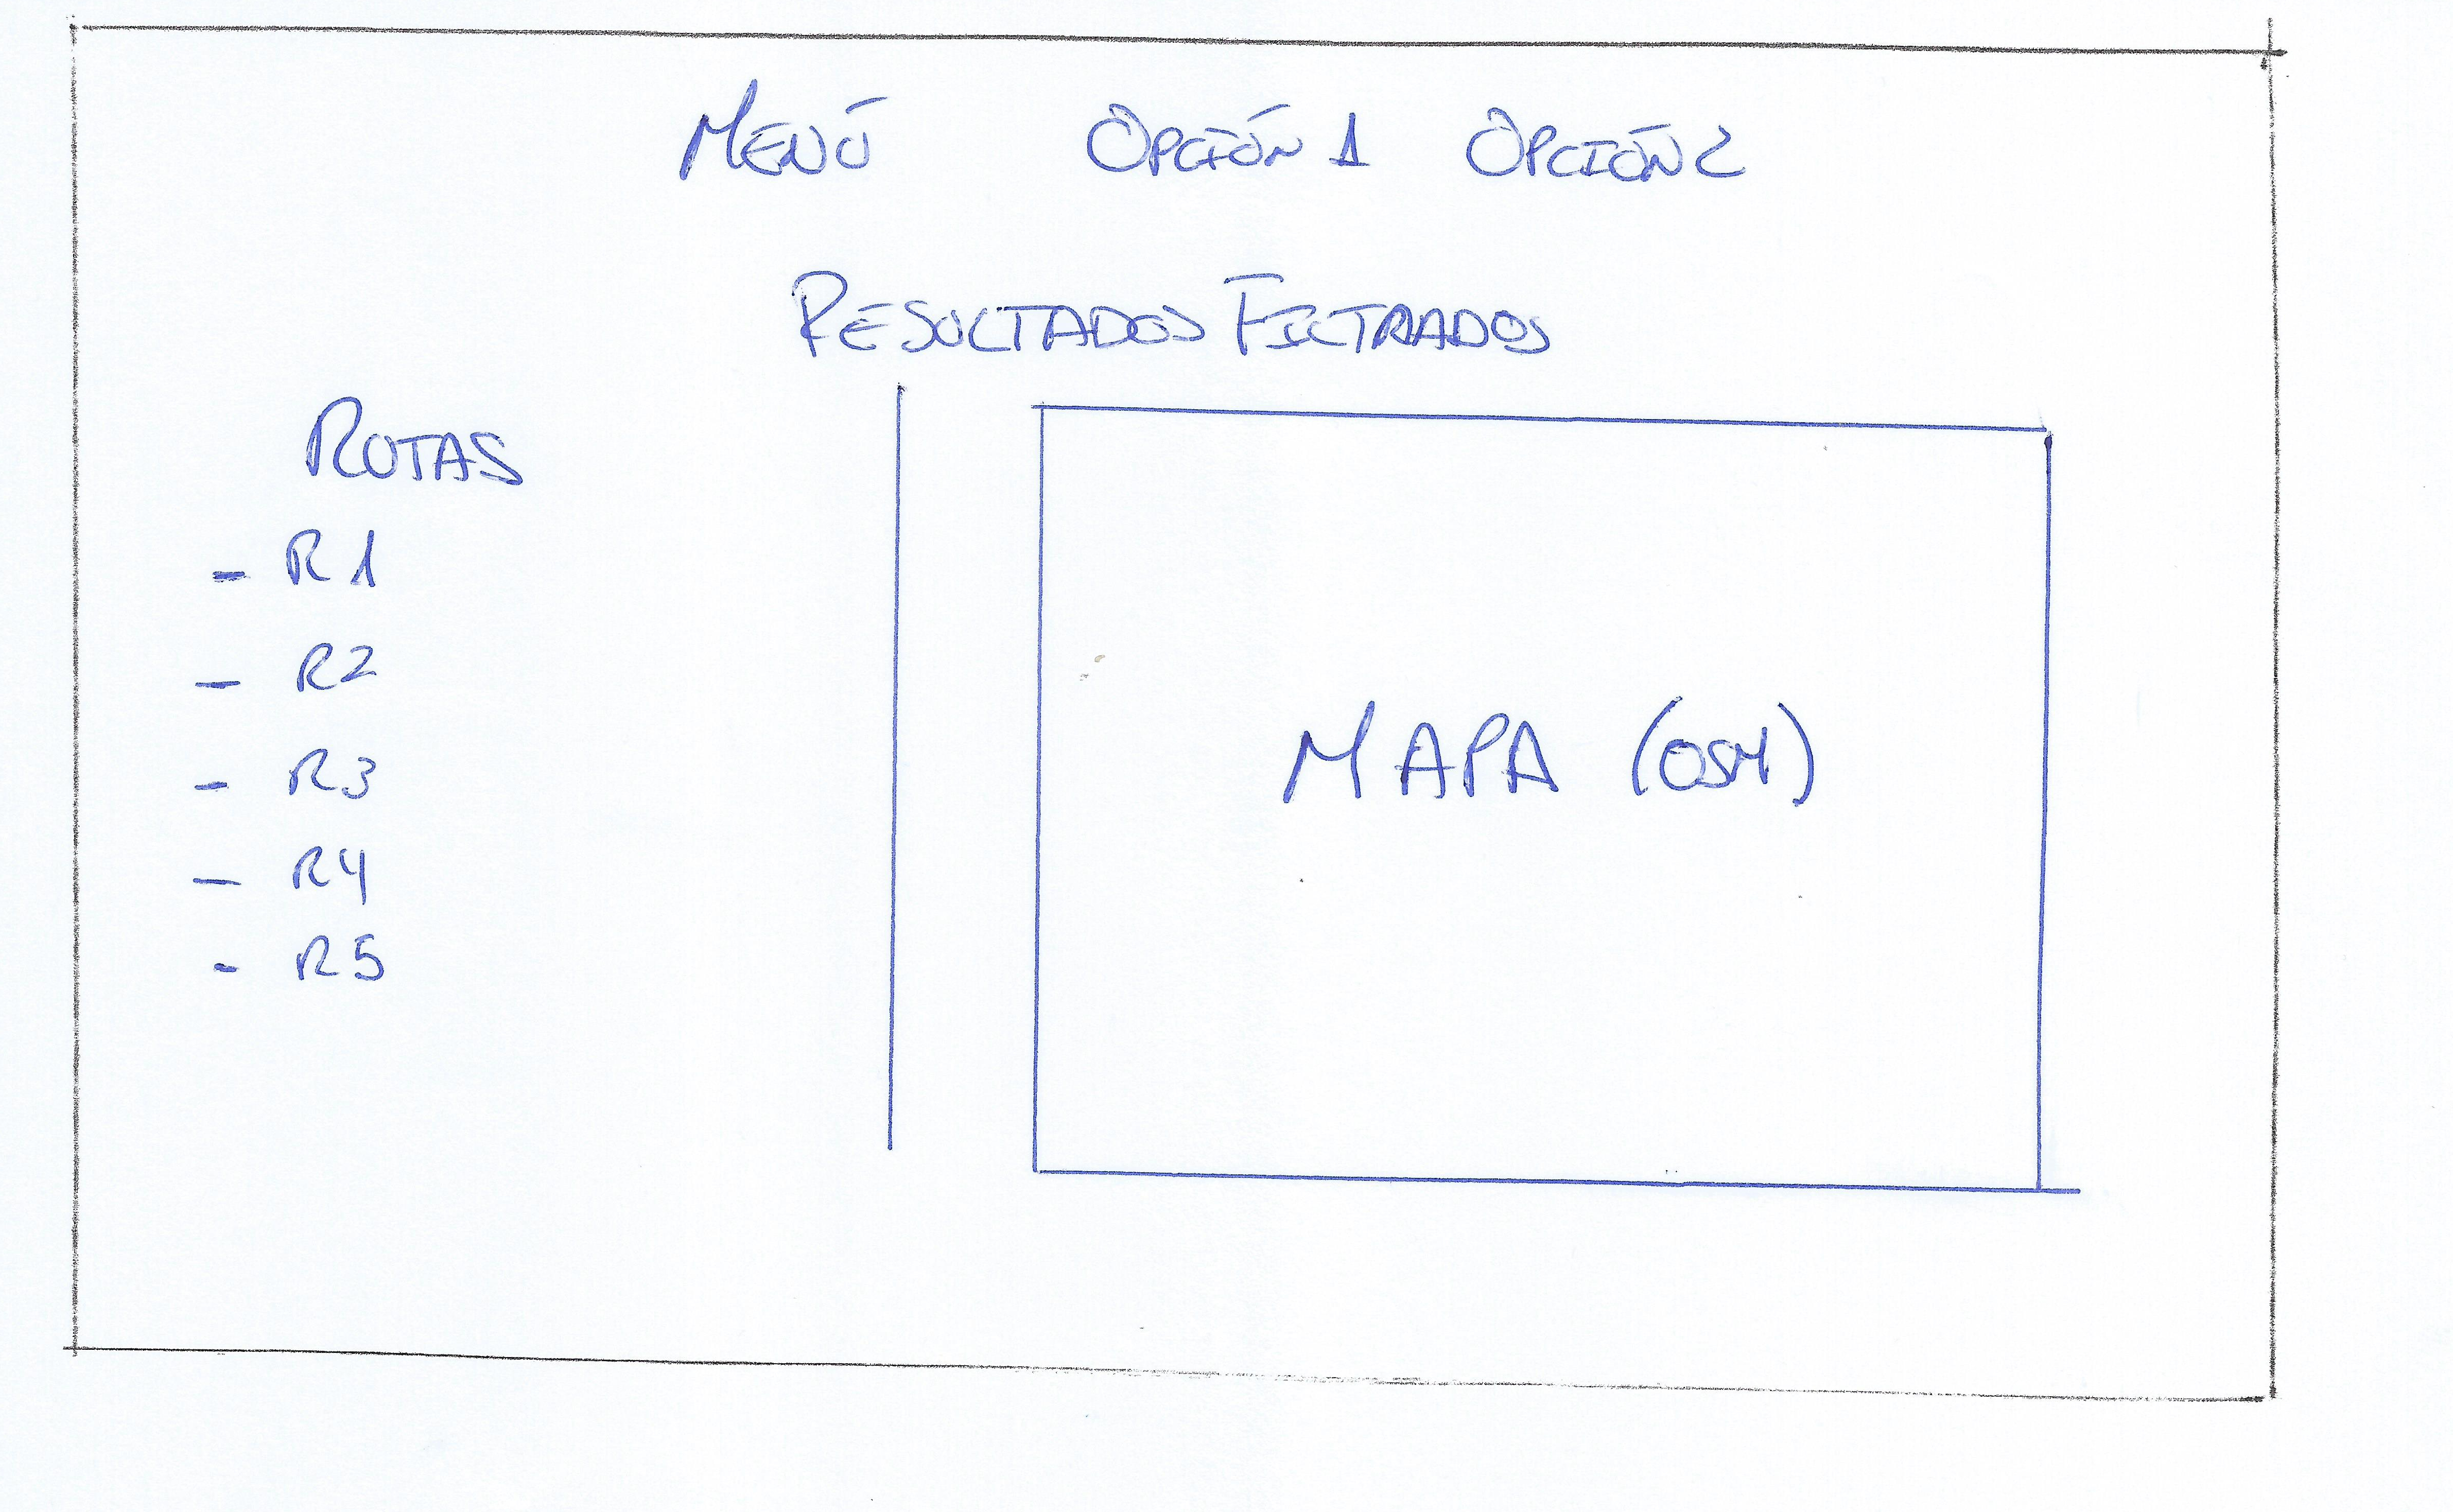
\includegraphics[width=0.6\textwidth]{../img/osmosis_descarga_mapa/mapa.jpg}
  \caption{Países mapeados de Sudamérica}
  \label{pais}
\end{figure}

\subsubsection{Extracción de una ciudad}
Para extraer una ciudad del plano que se acaba de descargar, se ha de abrir la consola del sistema y hacer uso del fichero de la aplicación Osmosis. Se necesitarán los siguientes argumentos (entre paréntesis las coordenadas que serán usadas en el caso de Aracaju):
\begin{itemize}
	\item Nombre del fichero de entrada: se seleccionará el fichero de extensión osm sobre el que se obtendrá el recorte del mapa.
	\item Coordenada GPS que indique la parte \textbf{superior} del segmento de mapa que se va a recortar (-36.441).
	\item Coordenada GPS que indique la parte \textbf{izquierda} del segmento de mapa que se va a recortar (-11.0367).
	\item Coordenada GPS que indique la parte \textbf{inferior} del segmento de mapa que se va a recortar (-37.6971).
	\item Coordenada GPS que indique la parte \textbf{derecha} del segmento de mapa que se va a recortar (-10.537).
	\item Nombre del fichero de salida: se dará nombre al fichero de salida con extensión osm.
\end{itemize}

El comando a teclear incluirá los siguientes parámetros:
\begin{itemize}
	\item rb: permite leer el contenido del fichero pbf descargado.
	\item bb: permite extraer los datos indicados en la caja definida por las coordenadas geográficas indicadas a continuación.
	\item top: coordenada geográfica superior.
	\item right: coordenada geográfica derecha.
	\item bottom: coordenada geográfica inferior.
	\item left: coordenada geográfica izquierda.
	\item wx: permite escribir los datos en un fichero osm.
\end{itemize}

Una vez descritos los parámetros y valores necesarios, se ejecuta el comando de la siguiente forma:

osmosis --rb /home/rs/osmdata/brazil-latest.osm.pbf --bb top=-36.441 left=-11.0367 bottom=-37.6971 right=-10.537 --wx /home/rs/osmdata/aracaju.osm

Una vez lanzado el comando, se verá la siguiente salida por consola:

\begin{figure}[h]
  \centering
    \includegraphics[width=0.6\textwidth]{../img/osmextract/resultado.jpg}
  \caption{Impresión en consola del resultado del comando.}
  \label{puntosGeograficos}
\end{figure}

\subsection{Carga de mapas OSM en PostGIS}
Una vez extraída la sección de mapa correspondiente a Aracaju se ha de cargar en PostGIS para poder hacer uso de toda su información posteriormente.

\subsection{osm2pgsql}
``osm2pgsql'' es una herramienta que permitirá la carga de los datos obtenidos mediante Osmosis en PostGIS. Antes de comenzar, se ha de instalar siguiendo los pasos indicados en su página de referencia (enlace: \url{http://wiki.openstreetmap.org/wiki/Osm2pgsql}). Los parámetros que la herramienta necesita para su correcto funcionamiento son:

\begin{itemize}
	\item s: habilita el modo ``slim'', recomendado en la guía de referencia.
	\item U: indica el usuario de la Base de Datos. En este caso: ``rs''.
	\item -d: indica la Base de Datos sobre la que se cargará el mapa. El valor debe ser ``rutassemanticas''.
	\item nombre del fichero: inmediatamente después del nombre de la Base de Datos, se indica la ruta al fichero que contiene el mapa. Se seleccionará el fichero de extensión OSM obtenido en el paso previo: ``aracaju.osm''.
\end{itemize}

El comando queda así:

osm2pgsql -s -U rs -d rutassemanticas /home/rs/osmdata/aracaju.osm

Una vez finalice, se crearán algunas tablas como ``planet\_osm\_nodes'', ``planet\_osm\_rels'' o ``planet\_osm\_ways''. Si ya existían, se añadirá el nuevo contenido.


\subsection{QGIS}
QGIS es una herramienta de información geográfica libre y de código abierto que permite conexiones con PostgreSQL y visualización de los datos obtenidos sobre un mapa físico. También permite la obtención de información geográfica desde Open Street Maps. De esta forma se pueden superponer rutas/trazas obtenidas desde las tablas de la Base de Datos con los mapas de Open Street Maps.

Para instalar QGIS desde ubuntu se han de seguir los pasos mostrados a continuación:

El primer paso es añadir la ruta a los ficheros fuente de QGIS en el fichero ``sources.list'', para ello se puede abrir dicho fichero con el editor nano. Se encuentra en la siguiente ruta: ``etc/apt/''.
Las líneas a añadir son las siguientes y pueden ser incluidas en la parte final del fichero:
\begin{lstlisting}
deb http://qgis.org/debian xenial main
deb-src http://qgis.org/debian xenial main
\end{lstlisting}

Ahora se puede proceder a la instalación de QGIS sobre el Sistema Operativo:

\begin{lstlisting}
apt install qgis python-qgis qgis-plugin-grass
\end{lstlisting}

Una vez instalado, se puede configurar una conexión contra la Base de Datos instalada y configurada anteriormente. Para ello se ha de clicar en el icono de PostgreSQL ubicado en la columna central izquierda. Para ello se han de indicar valores como:

\begin{itemize}
\item \textbf{nombre:} valor que se dará al nombre de la conexión.
\item \textbf{servidor:} servidor contra el que se realizará la conexión. En este caso será el servidor local.
\item \textbf{ de datos:} la Base de Datos de la que serán obtenidos los datos.
\item \textbf{Autenticación:} nombre de usuario y contraseña  del usuario de PostgresQL usado para obtener la información.
\end{itemize}

Otro de los aspectos importantes a tener en cuenta es la facilidad que brinda al usuario para descargar contenido en formato indicando una zona determinada mediante coordenadas geográficas. Esta característica ofrece el mismo resultado que el recorte del mapa de Brasil realizado con Osmosis. A continuación, se muestra un ejemplo con los mismos datos.

\subsubsection{Descarga de contenido OSM con QGIS}
Para comenzar, se ha de acceder a la sección ``Vectorial'', después, situar el cursor sobre ``OpenStreetMaps'' y clicar sobre ``Descargar datos'' (Figura \ref{vectorial}).


\begin{figure}[h]
  \centering
    \includegraphics[width=0.8\textwidth]{../img/qgis/descarga.jpg}
  \caption{Descarga de datos desde QGIS}
  \label{vectorial}
\end{figure}

A continuación se indicarán las coordenadas sobre las que se desea obtener los datos. En la Figura \ref{datos} se indican sus valores, son los mismos que los usados en Osmosis. Además, se ha de seleccionar un fichero destino. En este caso, se aprecia que es el mismo que el descargado mediante Osmosis.

\begin{figure}[h]
  \centering
    \includegraphics[width=0.8\textwidth]{../img/qgis/datos_3.jpg}
  \caption{Valores introducidos para la búsqueda de datos en QGIS}
  \label{datos}
\end{figure}

\begin{figure}[h]
  \centering
    \includegraphics[width=0.8\textwidth]{../img/qgis/exito_2.jpg}
  \caption{Éxito en la descarga de los datos.}
  \label{exito}
\end{figure}
Por último, se mostrará un mensaje de éxito si todo ha salido correctamente (Figura \ref{exito}).

Ahora se cuenta con el mismo fichero de extensión OSM y será posible su carga en PostGIS de la misma forma que se ha mostrado anteriormente.

Para obtener más información sobre QGIS se puede acceder al siguiente enlace: \url{http://www.qgis.org/es/docs/index.html}.



\section{\textit{Data cleaning}}
En esta sección se describe el proceso de \textit{data cleaning} o limpieza de datos aplicado a todas las rutas que se encuentran alojados en la Base de Datos.

\subsection{Origen de datos}
Antes de comenzar a describir el proceso de limpieza aplicado, se ha de tener en cuenta la procedencia de los datos usados para el presente Trabajo de Fin de Máster. El problema inicial al que hacer frente ha sido la falta de datos propios como punto de partida, por tanto, se ha tenido que realizar una búsqueda en distintos sitios de Internet para conseguir un conjunto de datos lo más fiables posible y con la estructura adecuada. Se han establecido una serie de condiciones indispensables que el dataset ha de cumplir:
\begin{itemize}
\item \textbf{Coordenadas geográficas:} cada coordenada ha de contar con una latitud y longitud separadas en dos campos.
\item \textbf{Marca de tiempo:} cada una de las coordenadas geográficas incluidas ha de contar con una marca de tiempo que permita localizar la coordenada en un espacio temporal concreto (un día, una semana, etc.).
\item \textbf{Altitud:} para que la coordenada geográfica sea más precisa, debe contar con su altitud.
\item \textbf{Diferenciación de rutas:} de igual manera que una coordenada geográfica se ha de poder diferencia de la siguiente, cada ruta incluida en el dataset ha de poder ser diferenciada del resto. Es importante que cada una de las rutas se diferencien mediante un identificador único o se encuentren en ficheros separados.
\end{itemize}

Algunos de los sitios donde se pueden buscar este tipo de dataset incluyen páginas como el repositorio de Machine Learning de la Universidad Irvine de California (\url{http://archive.ics.uci.edu/ml/}). Donde se pueden encontrar los últimos dataset subidos o un buscador para poder encontrar el dataset buscado. En esta página se han encontrado y valorado dos conjuntos de datos.

\subsubsection{Taxi Service Trajectory}
El primer dataset encontrado ha sido el correspondiente a distintos trayectos en taxi sobre la ciudad de Oporto (Portugal). Este dataset se compone de un amplio fichero csv con información como el tipo de llamada realizada a la compañía de taxis, el taxi que ha respondido a la misma, la fecha y hora a la que se produjo la llamada y el conjunto de coordenadas geográficas tomadas durante el trayecto.

Aunque el conjunto de los datos parece interesante en un primer momento, no se cuenta con un indicador temporal por cada coordenada y los hace inviables para su posterior uso, siendo este el motivo por el que se ha descartado el uso de este conjunto de datos.

Este dataset puede ser descargado desde el siguiente enlace: \url{https://archive.ics.uci.edu/ml/datasets/Taxi+Service+Trajectory+-+Prediction+Challenge,+ECML+PKDD+2015}.

\subsubsection{GPS Trajectories Data Set}
El segundo de los conjuntos de datos analizados ha sido el correspondiente a las rutas realizadas por un conjunto de usuarios en la ciudad de Aracaju (Brasil) en taxi o autobús. Estos datos se encuentran divididos en dos ficheros csv. El primero de los ficheros cuenta con un identificador único de usuario, de esta forma se puede conocer qué usuario ha tomado cada ruta, un indicador de velocidad de la ruta (inicialmente no necesario), un campo de tiempo, uno de distancia recorrida, algunos de calificación de la ruta (rating) y por último, uno indicando la línea de autobús en la que se ha realizado el trayecto.

El segundo de los ficheros incluye cada una de las coordenadas geográficas correspondientes a cada ruta y su asociación al usuario que la ha tomado.

Aunque inicialmente fue uno de los dataset tenidos en cuenta, se ha desechado por no contener un número elevado de rutas que permitiese una mayor aleatoriedad en los datos.

Este dataset puede ser descargado desde el siguiente enlace: \url{https://archive.ics.uci.edu/ml/datasets/GPS+Trajectories}.

\subsubsection{Geolife}
El dataset seleccionado ha sido el denominado Geolife GPS Trajectories. Este dataset pertenece al repositorio que mantiene Microsoft. Este conjunto de datos viene acompañado por un documento en el que se indica cómo se han obtenido los datos, cuál es su estructura, etc. Se menciona que los datos han sido recolectados por unos 180 usuarios, en su mayoría en la ciudad de Pekín (China) pero también existen datos de viajes a otras ciudades o, incluso, a otros países.

En el dataset se incluye una carpeta por cada usuario y en cada carpeta se puede encontrar un fichero que toma su nombre de la marca de tiempo de la primera coordenada de cada ruta. Por tanto, puede que un usuario cuente con un único fichero, indicando así que solo ha realizado una ruta, o que cuente con múltiples ficheros en los que se almacenan distintas rutas.

Cada fichero contiene una línea por cada coordenada geográfica obtenida. Esta línea contiene distinta información: un par latitud longitud, que permite situar la coordenada geográfica sobre un plano, su altitud y su marca temporal (entre otras). Esta estructura hace que la diferenciación de las rutas sea sencilla ya que se encuentran separadas por usuarios y marca temporal en la que ha sido tomada. Debido a esto, este conjunto de datos es el que ha sido finalmente elegido y volcado a la Base de Datos.

Finalmente, comentar que otras universidades como la de St Andrews (\url{https://uk.crawdad.org/}) también prestan sus dataset aunque, en esta ocasión, no se ha revisado su repositorio en profundidad.


\subsection{Proceso de limpieza}
Aunque los datos provistos por el dataset de Microsoft son fiables, se ha implementado un proceso de limpieza de los mismos para poder afinar todavía más los resultados.

Se ha comentado en la sección anterior que este dataset cuenta con diferentes carpetas en las que se incluyen los ficheros correspondientes a las rutas efectuadas por cada usuario. Uno de los problemas encontrados ha sido la continuidad de una ruta dentro de un mismo fichero. Para explicar esto, primero hay que saber, que cada coordenada tomada dentro de una misma ruta suele diferenciarse por una cantidad de tiempo (ya sean segundos o minutos) o espacial (metros) constante.

Poniendo un ejemplo, teniendo las siguientes coordenadas geográficas extraídas de un mismo fichero:

\begin{lstlisting}
40.004273,116.322334,87,2009-05-17,22:22:16
40.004285,116.322334,87,2009-05-17,22:22:21
40.004323,116.32235,8.,2009-05-17,22:22:26
40.004387,116.322366,91,2009-05-17,22:22:31
40.004371,116.322317,91,2009-05-17,22:22:36
40.00441,116.322294,92,2009-05-17,22:22:41
40.004435,116.322279,102,2009-05-17,22:22:46
40.004451,116.322241,120,2009-05-17,22:22:51
40.004214,116.322215,110,2009-05-17,22:35:46
40.004171,116.322241,108,2009-05-17,22:35:51
40.004125,116.322269,108,2009-05-17,22:35:56
40.004107,116.322301,105,2009-05-17,22:36:01
40.004132,116.32232,103,2009-05-17,22:36:06
40.004154,116.32232,103,2009-05-17,22:36:11
40.004192,116.322331,105,2009-05-17,22:36:16
40.004248,116.32235,109,2009-05-17,22:36:21
\end{lstlisting}

Se puede observar que cada punto geográfico es recolectado cada cinco segundos, aproximadamente. Teniendo esto en cuenta, se aprecia un salto importante entre la octava y la novena coordenada. En concreto, hay un salto de 12 minutos y 55 segundos. Esta diferencia contrasta con los cinco segundos transcurridos entre cada toma de tiempo. Por tanto, se puede pensar que ha ocurrido algún problema en la toma de datos o que se tratan de rutas diferentes aunque se encuentren en el mismo fichero. En este caso, como se trata de un salto importante sobre las mediciones tomadas, se realiza un corte en la ruta y se tratará como dos rutas diferentes.

Este pequeño ejemplo muestra el problema que puede ocurrir con el resto de las rutas disponibles en los ficheros del dataset. Se ha implementado un algoritmo para poder separar las rutas que, por tiempo o diferencia geográfica, parezcan pertenecer a dos o más rutas diferentes. Este algoritmo tiene en cuenta la mediana, tanto de la diferencia en términos de tiempo como de espacio.


El algoritmo comienza obteniendo todas las rutas de la Base de Datos y generando un mapa cuya clave es el identificador del usuario y valores las rutas del mismo. Después se recorre cada una de las rutas y se calcula una primera mediana (el usuario puede indicar si quiere la mediana sobre las marcas temporales o sobre las coordenadas geográficas). En base a esta primera mediana se empieza a analizar la ruta, siendo el siguiente paso, el cálculo de la diferencia temporal o geográfica entre cada dos de las coordenadas. Una vez obtenida esta lista de diferencias se comparará con la mediana obtenida anteriormente. En el caso de que no existan diferencias significativas, la ruta se mantendrá tal cual en la Base de Datos. Si, por el contrario, una posición de la lista contiene una diferencia apreciable, la ruta quedará separada, inicialmente, en dos tramos. El primer tramo se mantendrá en la Base de Datos pero el segundo tramo será re analizado calculando una nueva mediana y repitiendo el proceso descrito. Al final se podrán obtener varias rutas a partir de la inicial actualizando la Base de Datos con las nuevas rutas obtenidas.

Este algoritmo también es aplicable a ficheros de texto, que una vez procesados, generarán nuevas rutas en las tablas de la Base de Datos.